\chapter{Diseño del protocolo LoRaLAN}\label{chap:4}

En este capítulo se especifica el protocolo LoRaLAN. En primer lugar, se presentan su topología y los principios que han guiado su diseño. Posteriormente, se detallan todas las decisiones de diseño tomadas sobre el protocolo. Los repositorios que contienen el código están todos en el Anexo \ref{anexo:repos}.


\section{Visión general}

\textbf{LoRaLAN} es un protocolo de comunicación para redes de área local construido directamente sobre la capa física LoRa \cite{semtech_sx1276}. Define los mecanismos de las capas de enlace y de red necesarios para gestionar una red de un solo salto, incluyendo la delimitación y el direccionamiento de tramas, el acceso al medio, la fiabilidad de las comunicaciones, la asociación de dispositivos y la seguridad.

La red adopta una topología en \textbf{estrella}, con un único gateway y hasta 32 nodos en esta versión. Todos los nodos tienen al gateway en el otro extremo, por lo que los nodos no se comunican entre sí. Los dos roles que intervienen son los siguientes:

\begin{itemize}
\item \textbf{Nodo}: Es el dispositivo final. Gestiona la lógica de negocio de la aplicación correspondiente, se asocia al gateway, le envía eventos y telemetría y responde a sondeos e instrucciones cuando el gateway se lo solicita.

\item \textbf{Gateway}: Se encarga de coordinar la red. Permite la unión de nodos a la red, los sondea por turnos, difunde la hora, recibe sus eventos y les envía órdenes. Además, es el punto de unión con el exterior, puesto que la aplicación que se ejecuta sobre él traduce entre la red LoRaLAN y los sistemas a los que sirve (un servidor HTTP o un \textit{broker} MQTT, por ejemplo), aunque dicha traducción no forma parte del protocolo.
\end{itemize}

El diseño se ha guiado por los siguientes principios o condiciones:

\begin{enumerate}

\item \textbf{Cada byte cuenta}: Una trama ocupa el canal durante decenas de milisegundos y el tiempo de transmisión está regulado, por lo que la cabecera se reduce a 7~bytes y el cifrado no añade relleno. De esta manera se intenta disminuir la probabilidad de colisión además de optimizar al máximo el duty cycle.

\item \textbf{El gateway tiene capacidad de manejar el tráfico de dos formas}: El tráfico periódico lo ordena el gateway mediante una ventana de sondeo. Cada cierto periodo de tiempo el gateway pregunta a los nodos y estos responden con la información correspondiente. Este método de comunicación convive con eventos urgentes que los nodos emiten sin esperar turno, tras escuchar el canal para evitar colisiones.

\item \textbf{Los dispositivos escuchan siempre}: Excepto cuando transmiten, los nodos y el gateway permanecen en recepción continua. Se trata de una decisión coherente con dispositivos conectados a la red eléctrica, como los del caso de uso, donde se puede renunciar, en cierto modo, al bajo consumo.

\item \textbf{Un evento inmediato no se puede perder}: Todo evento que requiere confirmación termina con un resultado explícito para la aplicación del nodo. Para ello, se disponen mecanismos de repetición de mensaje y/o escucha previa en caso de estar el canal ocupado para evitar colisión.

\item \textbf{Fallo en cerrado}: Si la criptografía no está disponible el dispositivo no transmite ni acepta ningún paquete.

\item \textbf{El protocolo no tiene funciones de la capa de aplicación}: El protocolo no interpreta la carga útil, que pertenece a la aplicación.
\end{enumerate}

\section{Formato de paquete}\label{sec:trama}

Todos los paquetes comparten la misma estructura: una cabecera de 7~bytes, una carga útil de 0 a 64~bytes y un código de integridad de mensaje (MIC) de 4~bytes. La trama completa mide entre 11 y 75~bytes y viaja como carga útil de la trama física LoRa, que añade su propio preámbulo, su cabecera y su CRC. En la Figura~\ref{fig:loralanDentroLora} se puede apreciar cómo se encapsula LoRaLAN dentro de LoRa.

\begin{figure}[h]
    \centering
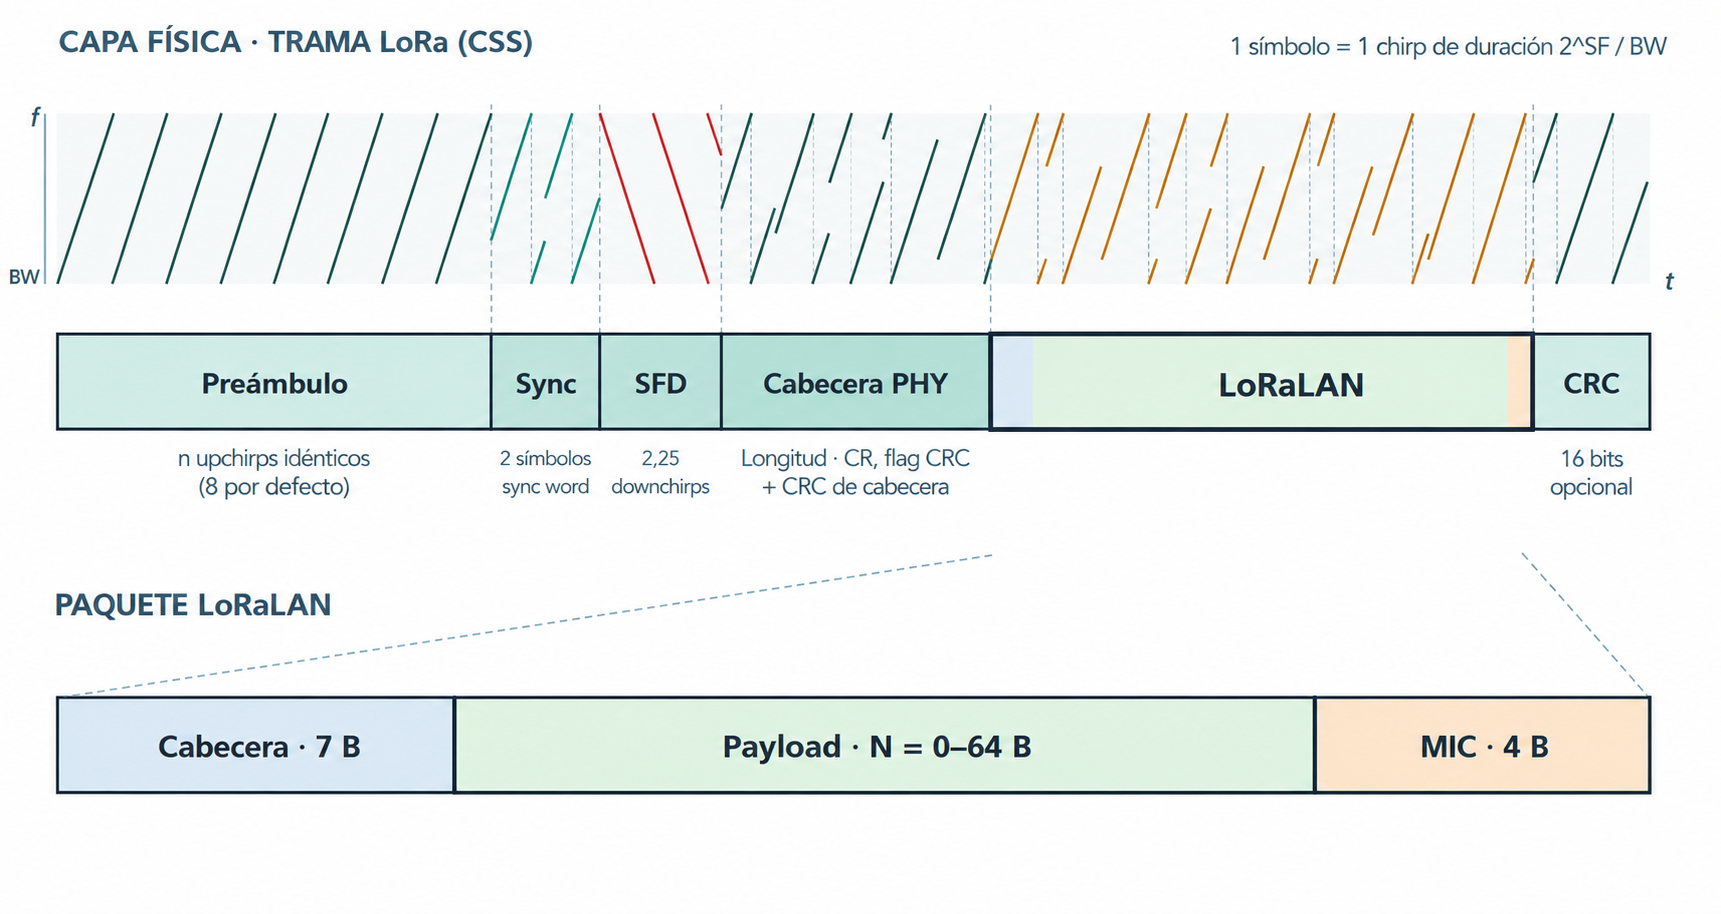
\includegraphics[width=1\linewidth]{./imagenes/loralanDentroLora.png}
    \caption{Encapsulación de paquete LoRaLAN dentro de la trama LoRa. }
    \label{fig:loralanDentroLora}
\end{figure}

\subsection{Cabecera}

En la figura~\ref{fig:loralancabecera} se muestra el formato del paquete y se desglosa la cabecera que llevan los paquetes tal y como viajan por el aire.

\begin{figure}[h]
    \centering
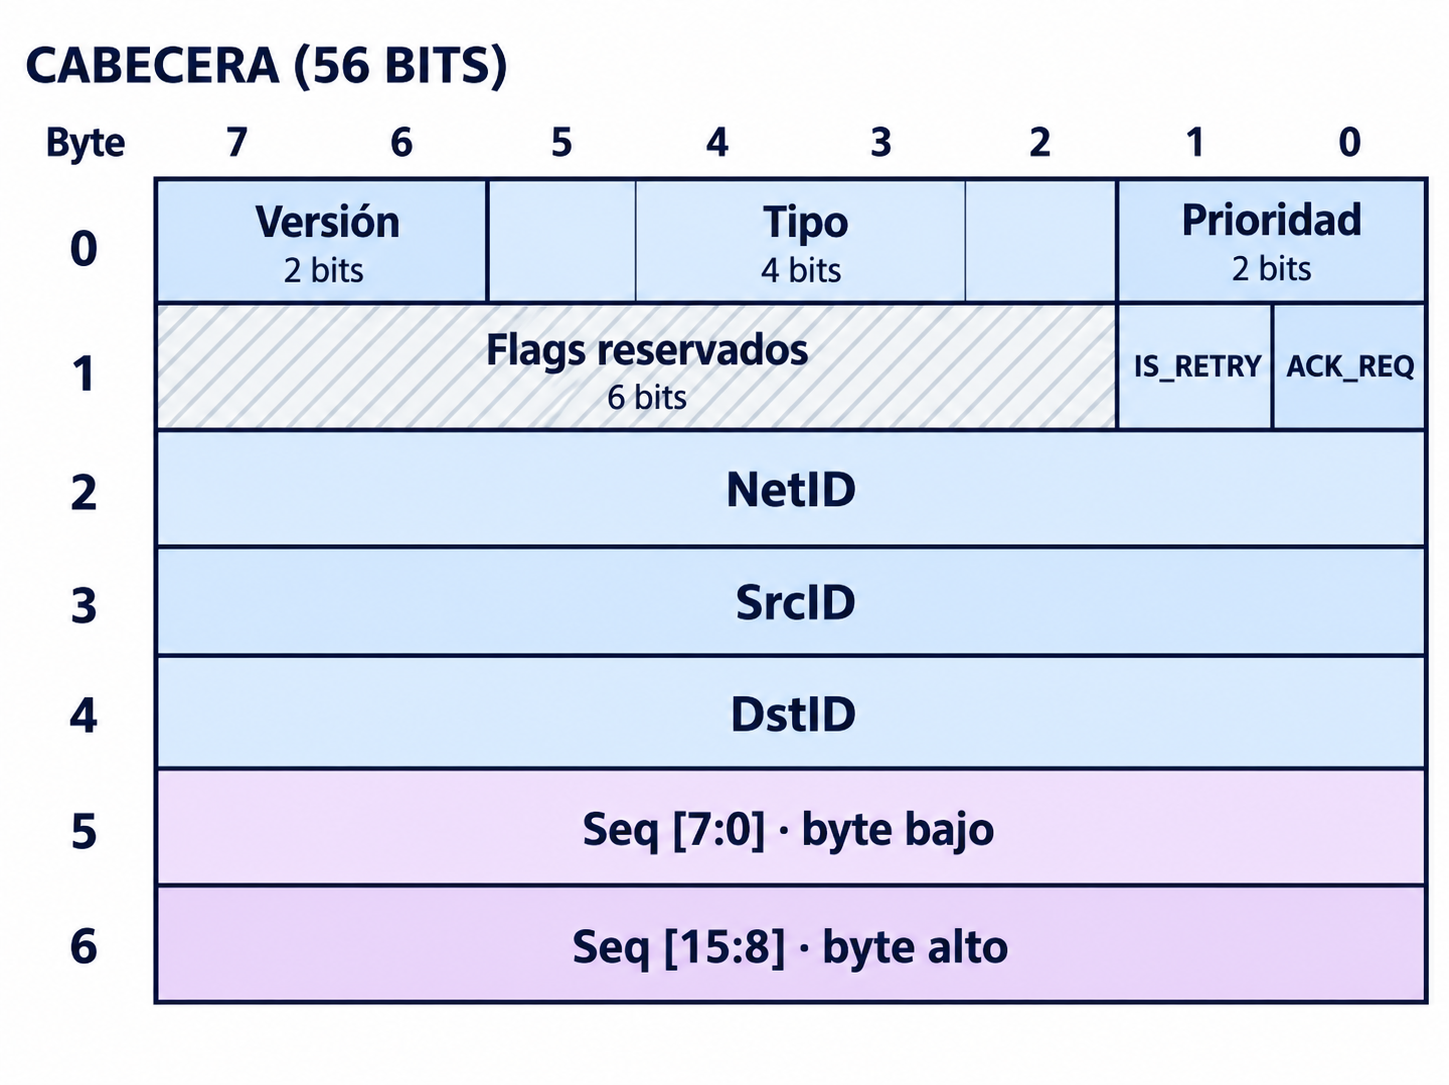
\includegraphics[width=0.8\linewidth]{./imagenes/cabecera.png}
    \caption{Campos de la cabecera de paquete LoRaLAN. }
    \label{fig:loralancabecera}
\end{figure}

En primer lugar se reservan 2 bits para indicar la \textbf{versión del protocolo} que se está utilizando. De esta forma, se permite que el protocolo pueda mejorarse y que puedan existir hasta cuatro versiones con distintas propiedades en un futuro.

El siguiente campo que aparece es el campo \textbf{tipo}, al que se asignan 4 bits. Este campo indica qué tipo de paquete se envía. Puede haber hasta 16 tipos de paquetes, aunque hasta el momento solo se han definido nueve.

Los nueve tipos de mensaje definidos, que se muestran en la Tabla~\ref{tab:tipos}, cubren el ciclo de vida completo de la red.
\begin{table}[H]
\centering
\caption{\label{tab:tipos} Tipos de mensaje de LoRaLAN.}
\small
\begin{tabular}{|c|l|p{8.5cm}|}
\hline
\textbf{Cód.} & \textbf{Tipo} & \textbf{Descripción} \\
\hline
\texttt{0x01} & PUSH\_EVENT & Evento de aplicación, el nodo lo envía por iniciativa propia al gateway. \\
\hline
\texttt{0x02} & ACK & Confirmación de recepción de un paquete, que puede llevar código de confirmación dentro del propio paquete. \\
\hline
\texttt{0x03} & POLL & Sondeo periódico que emite el gateway preguntando a un nodo si tiene datos que enviarle. \\
\hline
\texttt{0x04} & POLL\_RESPONSE & Respuesta del nodo a un sondeo, con los datos de aplicación que tuviera pendientes. \\
\hline
\texttt{0x06} & TIME\_SYNC & Difusión de la hora del gateway para que los nodos sincronicen su reloj. \\
\hline
\texttt{0x07} & JOIN\_REQUEST & Solicitud de un nodo para asociarse a una red. \\
\hline
\texttt{0x08} & JOIN\_ACCEPT & Respuesta del gateway a la solicitud de asociación, con el identificador asignado al nodo. \\
\hline
\texttt{0x09} & LEAVE & Aviso del nodo de que abandona la red. \\
\hline
\texttt{0x0A} & CMD & Orden que el gateway envía a un nodo por iniciativa propia. \\
\hline
\end{tabular}
\end{table}


El código \texttt{0x05} está reservado, debido a que correspondía a un mensaje de descubrimiento sin claves (HELLO) de las primeras versiones, que se eliminó cuando su función quedó cubierta por la asociación autenticada. 

Cabe destacar que el ACK reutiliza el campo de secuencia con un significado distinto al del resto de tramas: no lleva un número propio, sino el de la trama que confirma, permitiendo al emisor emparejar cada confirmación con su envío.

El siguiente campo que aparece es el de \textbf{prioridad}. Para este campo se reservan 2 bits, con los que se completa el primer byte de la cabecera.

El campo Prioridad puede tomar los valores de prioridad baja (0), media (1) y alta (2). Actualmente es solo informativo.

A continuación, aparece el campo \textbf{Flags}. Este campo ocupa un byte, aunque actualmente solo utiliza los bits ACK\_REQUIRED e IS\_RETRY. Esta decisión mantiene la cabecera alineada a byte sin reducir el espacio destinado a tipos o prioridades. El coste adicional de mantener este byte es mínimo, mientras que los seis bits restantes quedan reservados para futuras extensiones. Estos deben permanecer a cero y cualquier trama que incumpla esta condición será descartada, de modo que la incorporación de nuevos indicadores requerirá implementar una nueva versión del protocolo.

El indicador ACK\_REQUIRED señala al receptor que debe confirmar el paquete con un ACK. Por otro lado, el indicador IS\_RETRY señala que el paquete es una retransmisión. Este bit es solo informativo ya que se puede deducir que es una retransmisión por el número de secuencia.  

El siguiente byte representa el \textbf{identificador de red}. Como su nombre indica, sirve para separar redes que funcionan en el mismo canal. Si un nodo recibe un paquete con un netId distinto al de su red, lo descarta.

Los siguientes bytes representan la \textbf{dirección de origen} y la \textbf{dirección de destino} de los paquetes. Esto quiere decir que se dispone de un total de 254 direcciones para nodos, ya que la dirección 255 (0xFF) corresponde a la dirección de broadcast y la dirección 0 (0x00) corresponde a la dirección del gateway. Aunque teóricamente 254 sería el máximo de nodos que podrían conectarse a la red, dicho máximo se reduce a las 32 entradas de la tabla de direcciones que puede mantener el gateway. Este valor resulta adecuado para la aplicación del caso de uso y, además, disminuye el tiempo que tarda el gateway en sondear a todos los nodos y reduce su ciclo de trabajo.

Por último, se dedican dos bytes al \textbf{número de secuencia}, que cada emisor incrementa en cada envío. Permite al receptor descartar duplicados y repeticiones. Al emisor le permite emparejar cada ACK con su envío, ya que el ACK devuelve el número de la trama que confirma. Se emplean 16~bits porque, con un solo byte, el contador daría la vuelta cada 256~tramas y una trama capturada volvería a parecer nueva al poco tiempo.

Respecto a los duplicados, una retransmisión llega al receptor cuando la trama original también llegó pero su ACK se perdió. El receptor detecta el duplicado por el número de secuencia y, en ese caso, no entrega los datos a la aplicación por segunda vez, pero sí vuelve a confirmar. Esto se aplica tanto en el gateway, con los eventos y las respuestas de sondeo, como en el nodo, con las órdenes.

\subsubsection{Carga útil y código de integridad (MIC)}

La carga útil se limita a 64~bytes, lo que mantiene un equilibrio entre capacidad y tiempo en el aire. Con SF7, 125~kHz, CR 4/5, 8~símbolos de preámbulo, cabecera explícita y CRC, el paquete máximo (75~bytes) ocupa el canal 133~ms y el mínimo (11~bytes), 41~ms, según las fórmulas de Semtech recogidas en el Anexo~\ref{anexo:toa}. En esta versión inicial se descarta aplicar fragmentación de paquetes.

Tras el último byte de datos se incluye el MIC (\emph{Message Integrity Code}), un código de cuatro bytes, obtenido con CMAC-AES-128\cite{rfc4493}, que cubre la cabecera completa y la carga útil cifrada en los mensajes que transportan datos de aplicación y en claro en el resto. Su cálculo requiere una clave que depende del interlocutor, como se detalla en el apartado~\ref{sec:integridad}.

Antes de cualquier otra comprobación, el receptor comprueba que el paquete esté bien formado, es decir, que su longitud esté entre 11 y 75~bytes, que la versión sea la vigente, que el tipo esté definido, que la prioridad sea válida y que los indicadores reservados estén a cero, y descarta la trama que no supere alguna de estas comprobaciones. La cabecera no incluye un campo de longitud, ya que la cabecera explícita de LoRa transporta la longitud de la carga protegida por su propio CRC, de modo que la longitud de los datos de aplicación se deduce de la longitud total recibida. Un paquete alterado en tránsito para alargarlo o recortarlo puede superar esta validación estructural, pero no la del MIC, puesto que el cambio de longitud altera los bytes cubiertos y la posición del propio código. 

Mediante el MIC se garantizan la integridad y la autenticidad del paquete, lo que permite descartar los paquetes que presentan modificaciones no autorizadas y verificar que el emisor es legítimo y posee la clave secreta.
\section{Gestión del direccionamiento y vinculación a redes}\label{sec:join}


\subsection{Asociación (JOIN)}

La asociación es el mecanismo mediante el cual un nodo se vincula a una red LoRaLAN para poder transmitir información y posee tres funciones: autenticar al nodo y al gateway mediante una clave maestra precompartida (denominada \textit{APPKEY}, de 128~bits), establecer una clave de sesión exclusiva de ese nodo y dar de alta al nodo en la tabla del gateway. Los pasos que se llevan a cabo son los siguientes:

\begin{enumerate}
\item El nodo genera un número aleatorio de 16~bits, denominado \textit{DevNonce}, y emite un paquete tipo JOIN\_REQUEST a la dirección de difusión con su tipo de dispositivo, dicho DevNonce y su identificador de fábrica (dirección MAC), empleando como dirección de origen la que desea obtener. Este paquete se autentica con la clave APPKEY.

\item El gateway verifica el MIC, localiza al nodo en su tabla por su identificador de fábrica o le asigna una dirección si no figura en ella, y deriva la clave de sesión a partir de la dirección asignada. Posteriormente, responde con un JOIN\_ACCEPT dirigido a esa dirección, que contiene la propia dirección asignada, el mismo DevNonce, un código de estado y el identificador de fábrica del nodo.

\item El nodo comprueba que el DevNonce y el identificador de fábrica devueltos coinciden con los suyos, lo que liga la respuesta a su petición, adopta la dirección asignada y deriva la misma clave por su cuenta. Finalmente, confirma con un ACK que ya va autenticado con la clave de sesión.
\end{enumerate}
 
De esta forma, la clave de sesión no viaja nunca por el aire, sino que en ambos extremos se calcula a partir de datos de los que se dispone. Si no recibe respuesta, el nodo repite la petición cada 5~segundos (valor configurable), con un DevNonce nuevo en cada intento. Para emitir un paquete JOIN\_REQUEST se realiza previamente una escucha del canal y, si este se encuentra ocupado, el intento se aplaza al siguiente periodo.

Cuando un nodo previamente asociado se reinicia, vuelve a solicitar la asociación. El gateway la acepta, deriva una clave nueva y reinicia el estado de esa sesión, incluido el control de secuencia. 

Si el gateway se reinicia, su tabla arranca vacía y deja de reconocer a los nodos que siguen considerándose asociados, de modo que descarta sus paquetes, por no disponer de su clave de sesión, y no los incluye en el sondeo. Para detectar esta situación, el nodo registra el instante del último paquete recibido con su clave de sesión (POLL, CMD o ACK) y, si transcurre un plazo (configurable) sin recibir ningún paquete destinado a él, da la sesión por perdida, borra su clave y vuelve a solicitar la asociación. Los paquetes TIME\_SYNC no se tienen en cuenta, puesto que se autentican con la clave maestra y un gateway reiniciado los sigue emitiendo. Dicho plazo debe superar, al menos, una vuelta completa de sondeo, cuya duración depende del número de nodos asociados.

\subsection{Asignación dinámica de direcciones}\label{sec:direcciones}

Cada nodo dispone de un \textbf{identificador de fábrica} de 6~bytes, la dirección MAC grabada en el microcontrolador, que viaja en el JOIN\_REQUEST y en el JOIN\_ACCEPT. Conviene no confundirlo con el DevNonce, cuyo papel es distinto. El identificador de fábrica es fijo y señala quién es el nodo, mientras que el DevNonce cambia en cada intento, lo que impide repetir una asociación capturada y garantiza que cada sesión tenga una clave distinta. Que el JOIN\_ACCEPT incluya también el identificador permite a cada nodo reconocer la respuesta que le corresponde aunque varios se asocien a la vez, como ocurre tras un corte de suministro general, por ejemplo.

Al recibir una petición, el gateway asigna la dirección aplicando las siguientes reglas, en este orden:

\begin{enumerate}
\item Si el identificador de fábrica ya figura en su tabla, devuelve la misma dirección, sea cual sea la que pida el nodo.

\item En caso contrario, concede la dirección que el nodo solicita como origen del JOIN\_REQUEST, siempre que no sea \texttt{0x00} (por defecto, sin preferencia), \texttt{0xFF} ni la del propio gateway y que no la ocupe otro nodo.

\item Si no puede concederla, asigna la dirección libre más alta, empezando por la 254. Si no queda ninguna, la petición se rechaza.
\end{enumerate}

La tabla de direcciones del gateway reside en memoria durante la ejecución, de modo que la persistencia la aporta el nodo, que guarda la dirección recibida en su memoria no volátil y la solicita de nuevo en cada asociación. La biblioteca se limita a ofrecer la dirección preferida como parámetro de configuración y la asignada como dato consultable, por lo que su almacenamiento se delega en la capa de aplicación. Con este reparto, un nodo recupera su dirección tanto si se reinicia el gateway, ya que la conserva en memoria y la pide al reasociarse, como si se produce un corte general, puesto que la lee de su memoria no volátil.

El protocolo ofrece un direccionamiento dinámico similar al que ofrece DHCP. Se aplica ofreciendo al nodo la dirección más alta disponible. De esta manera se reservan las direcciones bajas (1-127) para direccionamiento fijo. Es decir, los administradores de la red pueden asignar a un nodo una dirección de ese rango, de manera que el gateway le proporcionará al nodo la dirección deseada si se encuentra disponible.


\subsection{Baja (LEAVE)}

Un nodo abandona la red emitiendo un paquete LEAVE y esperando el ACK correspondiente. Tras recibirlo, borra su clave de sesión y deja de intentar asociarse hasta que su aplicación lo solicite. Si tras varias repeticiones no se recibe ACK, el nodo abandona la red de igual forma. La pérdida del LEAVE o de su ACK no deja a la red en un estado incoherente, ya que el gateway registra el instante del último paquete recibido de cada nodo y, si este no responde tras varias ventanas de sondeo, lo marca como inactivo.

Un nodo puede desaparecer porque se ha dado de baja, porque se ha apagado o porque ha quedado fuera de cobertura. En cualquiera de estos casos deja de responder a los sondeos y la aplicación puede considerarlo inactivo. No obstante, el gateway no lo retira por sí mismo del turno de sondeo, de modo que un nodo que desaparece sin que su baja llegue al gateway sigue consumiendo su turno para que pueda recuperarse si su ausencia es temporal.

\section{Acceso al medio híbrido}\label{sec:mac}

LoRaLAN aplica un esquema híbrido con dos modos complementarios, en línea con los trabajos sobre coordinación centralizada y escucha previa del canal revisados en el Capítulo~\ref{chap:2}.

\subsubsection{Modo POLL o sondeo dirigido por el gateway}\label{sec:poll}

El gateway recorre cíclicamente su tabla de nodos asociados y asigna un periodo de tiempo configurable que determina cuánto tiempo pasa entre que se consulta a un nodo y a otro. Para ello, cuando a un nodo le llega su turno, el gateway envía un POLL\_REQUEST a dicho nodo. El nodo interrogado contesta con un POLL\_RESPONSE, cuyo contenido se elige en el siguiente orden:

\begin{enumerate}
    
\item Los datos que la aplicación hubiera dejado preparados para el siguiente sondeo, o los de un evento cuya entrega por el modo PUSH no se confirmó, si los hay.

\item Datos que la aplicación genera en ese instante, si se registra una función para ello (sondeo bajo demanda). En el caso de uso de este trabajo se aplica a telemetría proporcionada por lectura de sensores y estado de relés.

\item En último lugar, una carga vacía, que sirve como señal de vida (Heartbeat).

\end{enumerate}

El POLL\_REQUEST no requiere confirmación, puesto que el propio POLL\_RESPONSE ya sirve como acuse de recibo. Por otro lado, la confirmación del POLL\_RESPONSE será necesaria o no, dependiendo de su contenido. Las respuestas vacías y las generadas bajo demanda, que transportan telemetría o estado que el siguiente sondeo vuelve a refrescar, se emiten una sola vez y sin confirmación, de modo que el ciclo habitual consta únicamente de dos paquetes: el POLL\_REQUEST y el POLL\_RESPONSE.

Por el contrario, los datos prioritarios se envían como una transmisión fiable que el gateway confirma, salvo que la aplicación indique lo contrario al encolarlos. El ciclo consta en ese caso de tres paquetes. El nodo retransmite la respuesta si la confirmación no llega y conserva los datos hasta recibirla, de manera que, si agota los intentos, los vuelve a enviar en el siguiente turno de sondeo.

Que el gateway elija el turno de cada nodo resulta la vía más eficiente para el tráfico rutinario, como la telemetría o el estado. Su principal desventaja es la latencia. Dados $N$ nodos y un intervalo de sondeo $T_{poll}$, cada nodo es interrogado cada $N \cdot T_{poll}$. Como el gateway emite un POLL en cada intervalo, $T_{poll}$ es el parámetro que fija el consumo de ciclo de trabajo del gateway y debe elegirse teniendo en cuenta dicho criterio.


\subsubsection{Modo PUSH: eventos asíncronos con CAD}

Un evento que no puede esperar a su turno, como un registro de asistencia, se transmite como PUSH\_EVENT. Para no interferir con una transmisión en curso de otro nodo o del gateway, el nodo escucha previamente el canal mediante la detección de actividad (CAD) del transceptor. El CAD está implementado por hardware en el transceptor LoRa utilizado, el SX1276 \cite{semtech_sx1276}. Con este diseño, se pueden dar tres casos:

\begin{enumerate}
\item Si el canal está \textbf{libre}, emite su transmisión.
\item Si el canal se encuentra \textbf{ocupado}, aplaza el intento aplicando un tiempo de retroceso (\textit{backoff}) exponencial con una componente aleatoria:
\begin{equation}\label{eq:backoff}
t_{espera} = t_{base} \cdot 2^{\min(k,\;k_{max})} + U(0,\;t_{jitter})
\end{equation}
donde $k$ es el número de escuchas fallidas del evento y $U$ una variable uniforme. Con los valores por defecto ($t_{base}=40$~ms, $k_{max}=5$, $t_{jitter}=50$~ms), la espera crece desde 80~ms hasta unos 1,3~s, y la componente aleatoria evita que dos nodos que han detectado la misma trama reintenten a la vez.

\item Si la escucha falla por un error de la radio, reintenta tras una espera fija y corta, de 60~ms.
\end{enumerate}

Un nodo mantiene un único evento pendiente de entrega. La aplicación no puede encolar otro evento hasta que el anterior se haya transmitido. Mientras existe una transmisión propia a la espera de confirmación, el nodo no realiza escuchas, dado que el CAD saca momentáneamente a la radio del modo de recepción y podría hacerle perder precisamente la confirmación que espera.


La escucha previa del canal se aplica \textbf{únicamente en los nodos} y solo a la primera emisión de cada PUSH\_EVENT y a cada JOIN\_REQUEST; si el canal está ocupado, el evento aplica el retroceso descrito y el JOIN espera a su siguiente intento. Las retransmisiones y el resto de tramas del nodo, así como todas las del gateway, se emiten sin escuchar.

Esta decisión es coherente con el rol del gateway como coordinador, puesto que es el único origen del tráfico descendente y él mismo provoca el ascendente del sondeo. Se entiende como tráfico ascendente (Uplink) a aquellos paquetes que van del nodo al gateway y descendente (Downlink) al tráfico que va desde el gateway a los nodos.

En contrapartida, un PUSH\_EVENT puede estar en el aire cuando el gateway emite un POLL o un TIME\_SYNC, en cuyo caso pueden perderse una o ambas tramas. Los reintentos permiten resolver las colisiones.

Aunque en esta versión el campo prioridad es informativo, los paquetes de tipo evento, confirmaciones y órdenes llevan un valor de prioridad alto, los paquetes relativos al sondeo una prioridad baja y prioridad media para paquetes que tratan la gestión de red (asociación, baja y sincronización). Esta decisión se hereda de una versión anterior en la que se planteaba que el gateway pudiera usar un planificador de colas para gestionar el tráfico de la red, como haría un switch o router para mantener la calidad del servicio (QoS).


\section{Fiabilidad}\label{sec:fiabilidad}

Los paquetes que llevan activado el indicador de confirmación requerida deben ser contestados con un ACK. El emisor aplica un esquema de parada y espera (\textit{stop-and-wait}): transmite el paquete, espera el ACK durante un plazo de 1200~ms por defecto y, si este no llega, retransmite hasta alcanzar un máximo de tres intentos en total. Cada retransmisión conserva el número de secuencia original y activa el indicador de retransmisión, lo que modifica la cabecera y obliga a recalcular el MIC. Cada dispositivo mantiene una única transmisión fiable en curso, mientras que las tramas que no piden confirmación se emiten una sola vez, sin esperar ningún ACK.

También se aplica otro mecanismo más simple. Si el transceptor informa de un fallo al transmitir, el envío se repite tras una pausa aleatoria de 30 a 180~ms, hasta tres veces, salvo en paquetes que no piden confirmación, que se intentan una única vez.

Respecto a los duplicados, una retransmisión llega al receptor cuando la trama original también llegó pero su ACK se perdió. El gateway detecta el duplicado por el número de secuencia y, en ese caso, \emph{no entrega los datos a la aplicación por segunda vez, pero sí vuelve a confirmar}.

Por otro lado, un PUSH\_EVENT podría agotar sus retransmisiones sin recibir confirmación. En ese caso, si la aplicación lo solicitó, sus datos no se descartan, sino que se guardan como carga del siguiente POLL\_RESPONSE, de modo que el evento pierde su carácter inmediato pero se garantiza su entrega en cuanto el gateway vuelve a interrogar al nodo. Dado que el gateway pudo recibir el evento original aunque se perdieran todas sus confirmaciones, los datos rescatados pueden llegar duplicados con otro número de secuencia, por lo que la aplicación debe reconocerlos por cualquiera de las dos vías y tolerar esa repetición.

Tanto si la confirmación llega como si se agotan los intentos, el nodo notifica a su aplicación el desenlace de cada evento, siendo esta la que decide qué hacer: mostrar un error, guardar el dato para más tarde o descartarlo.

Estos mecanismos presentan algunas limitaciones, puesto que ciertos conflictos, como los duplicados que puede generar el rescate por sondeo, se delegan en la capa de aplicación, y en otros casos la entrega no se pierde, pero se retrasa. Así, dado que cada dispositivo mantiene un único envío fiable en curso, los datos preparados que requieren confirmación no pueden salir en un sondeo que llegue mientras el nodo espera otro ACK, pero no se descartan, sino que se conservan para el sondeo siguiente.

\subsubsection{Confirmación con carga útil (ACK diferido)}\label{sec:ackdiferido}

Se han realizado algunas modificaciones pensando en el caso de uso. En este caso, cuando el nodo envía la tarjeta leída para procesar un fichaje, debe indicar al nodo si el fichaje se ha registrado correctamente o se ha rechazado, y además por qué. Esta decisión la toma el servidor.

Para cubrir esta necessidad se decide que la respuesta de la aplicación viaja dentro del propio ACK.

Cuando el gateway se configura con confirmación diferida, la recepción de un PUSH\_EVENT no genera el ACK automático. En su lugar, el protocolo entrega el evento a la aplicación del gateway y deja la confirmación en suspenso. Una vez que la aplicación dispone de la respuesta, la entrega al protocolo junto con el identificador del nodo y el número de secuencia del evento, y el protocolo emite el ACK con esa respuesta como carga útil. En el nodo la respuesta llega a la aplicación junto con el resultado del envío.

Para que este mecanismo sea compatible con los reintentos, el gateway guarda, por cada nodo, el estado de la confirmación de su último evento, que puede tomar tres valores:

\begin{itemize}
\item \textbf{Pendiente}: El evento se ha entregado a la aplicación y esta aún no ha respondido. Si llega una retransmisión del mismo evento, el gateway no contesta, ya que todavía no dispone de respuesta y el nodo volverá a intentarlo.
\item \textbf{Lista}: La aplicación ha respondido y el ACK se ha emitido. Además, el gateway \emph{conserva la respuesta}, de modo que si el ACK se pierde y el nodo retransmite, este recibe la misma respuesta sin que la aplicación vuelva a ser consultada.
\item \textbf{Ninguna}: No hay ningún evento en curso para ese nodo.
\end{itemize}

De este modo, un evento se procesa una sola vez aunque se transmita varias, y todas sus retransmisiones obtienen la misma respuesta. Si la aplicación entrega una respuesta cuando el evento ya no está pendiente (porque ha llegado otro posterior o porque el nodo se ha reasociado), dicha respuesta se rechaza.

%pero esto podría dar lugar a que no se envie la confirmación...

La respuesta debe emitirse antes de que venza el plazo de espera del nodo, que es de 1200~ms por defecto. El protocolo no impone cómo se consigue, de modo que es responsabilidad de la aplicación del gateway responder a tiempo, aunque sea con una respuesta provisional. En el Capítulo~\ref{chap:7} se describe cómo lo resuelve el sistema de fichaje.

Como alternativa a este mecanismo, se podría haber definido una confirmación negativa (NACK). Esta opción se descartó, ya que la distinción entre «aceptado» y «rechazado» pertenece a la aplicación, por lo que el protocolo debe transportar la respuesta sin interpretarla.

Otro detalle que cabe destacar es que la carga del ACK no se cifra, aunque el MIC, calculado con la clave de sesión, garantiza que procede del gateway y que no se ha alterado. Como cualquiera que escuche el canal tiene capacidad de leerla, no debe emplearse para datos confidenciales, sino para códigos de resultado breves.



\subsubsection{Sincronización temporal}

% REVISAR LA HORA PQ ES COMPLICADO PARA CREAR UNA HORA
El gateway difunde, con la periodicidad que indique el programador, un paquete TIME\_SYNC con una marca de tiempo de 32~bits en segundos, a partir de la cual cada nodo calcula y almacena su desfase respecto al reloj local sin modificarlo, de modo que la aplicación puede consultarlo para fechar sus datos o mostrar la hora. Este mecanismo es un servicio para la aplicación y no interviene en el acceso al medio, puesto que el sondeo de LoRaLAN es de pregunta y respuesta y un nodo transmite al recibir su POLL y no según su reloj, por lo que la pérdida de tramas TIME\_SYNC no afecta al funcionamiento de la red. Su resolución es de un segundo, ya que no tiene en cuenta el tiempo en el aire de la trama, y el valor difundido es el tiempo de funcionamiento del gateway y no la hora del día, cuya difusión exigiría ampliar la aritmética del nodo, que opera con milisegundos en 32~bits. Al tratarse de una trama de difusión, se autentica con la clave maestra, que es la única que comparten todos los nodos.

\section{Arquitectura de seguridad}\label{sec:seguridad}

El diseño de la seguridad asume de base que el canal es hostil \cite{chacko2018security}, puesto que cualquiera con un receptor LoRa en la misma frecuencia puede escuchar, capturar y reinyectar tramas LoRa. Se decide aprovechar el motor de aceleración hardware que ofrece el ESP32 \cite{babiuch2019esp32}, en dos modos: el modo contador para cifrar la carga útil con el algoritmo AES-128 y CMAC para autenticar paquetes y derivar las claves de sesión.

\subsubsection{Confidencialidad}

La carga útil de los paquetes que transportan datos de aplicación (PUSH\_EVENT, POLL\_RESPONSE y CMD) se cifra con AES-128 en modo contador (CTR) \cite{nist80038a} bajo la clave de sesión del nodo. Se ha elegido este modo porque convierte el cifrador de bloque en uno de flujo, de manera que el texto cifrado ocupa lo mismo que el original y la trama no crece, en coherencia con el primer principio de diseño.

%REVISAR SI EL NODO USA LA CLAVE DE NODO O LA CLAVE PRECOMPARTIDA.
El bloque inicial del contador se forma con el identificador de red, la dirección del emisor y el número de secuencia. La dirección del emisor es necesaria porque los dos sentidos del enlace comparten clave, y sin ella una trama del gateway y otra del nodo con el mismo número de secuencia emplearían el mismo flujo de cifrado.

El resto viaja en claro. La cabecera no puede cifrarse, ya que el receptor necesita leer el identificador de red y las direcciones para saber si la trama le concierne y con qué clave verificarla, y tampoco se cifran las tramas de gestión ni la carga del ACK, que solo contienen datos de control.

\subsubsection{Integridad y autenticidad}\label{sec:integridad}

El MIC ya descrito se calcula sobre la carga ya cifrada, de modo que el receptor lo verifica antes de descifrar y descarta cualquier trama que no lo supere sin llegar a procesarla (esquema \textit{Encrypt-then-MAC}). Con 4~bytes, el mismo tamaño que emplea LoRaWAN, la probabilidad de que una trama falsificada al azar sea aceptada es de $2^{-32}$, y cada intento le cuesta al atacante una transmisión completa.

La clave con la que se calcula depende del tipo de trama. Las de asociación usan la clave maestra, porque todavía no existe clave de sesión, y también la usa TIME\_SYNC, porque al difundirse a todos los nodos necesita una clave que todos compartan. El resto de tramas se autentica con la clave de sesión del nodo que interviene, por lo que el MIC se calcula en el momento de transmitir y no al construir la trama, y si no existe clave para el interlocutor, la trama no se emite ni se acepta.

\subsubsection{Derivación de claves de sesión}\label{sec:kdf}

La clave de sesión se obtiene durante la asociación aplicando CMAC con la clave maestra sobre una etiqueta fija, el identificador de red, la dirección asignada al nodo y el DevNonce:

\begin{equation}
K_{sesion} = \mathrm{CMAC}_{APPKEY}\big(\,\texttt{LLK} \parallel id_{red} \parallel id_{nodo} \parallel DevNonce\,\big)
\end{equation}

Al intervenir la dirección y el DevNonce, cada nodo tiene una clave distinta que además cambia en cada asociación, y como CMAC no es reversible, conocer la clave de un nodo no permite deducir la de otro ni la clave maestra. La etiqueta fija evita que la entrada de la derivación pueda coincidir con la de una trama de asociación autenticada con la misma clave. La primera versión del protocolo no cumplía esta propiedad, ya que derivaba las claves con una función lineal, se sustituyó para que fuera más robusta.

\subsubsection{Protección frente a repetición}\label{sec:antirepeticion}

Un paquete capturado y reinyectado sin modificar conserva un MIC válido, por lo que solo puede rechazarse si el receptor recuerda qué números de secuencia ha aceptado ya. Para ello, cada receptor guarda, por cada interlocutor, el último número aceptado y un mapa de 64~bits que indica cuáles de los 64~números anteriores ha recibido. Una paquete se acepta solo en alguno de estos dos casos:

\begin{itemize}
\item Si su número avanza respecto al último aceptado hasta media escala, es decir, entre 1 y 32\,767~posiciones teniendo en cuenta la vuelta del contador. En ese caso pasa a ser el último aceptado y el mapa se desplaza.

\item Si es uno de los 64~números anteriores y el mapa indica que todavía no se ha recibido, lo que permite aceptar tramas que llegan fuera de orden.
\end{itemize}

Cualquier otro número se considera una repetición o una trama demasiado antigua y se rechaza. Admitir avances de hasta media escala permite recuperar la comunicación tras una racha larga de pérdidas y, al mismo tiempo, distinguir sin ambigüedad una trama nueva de una antigua cuando el contador da la vuelta. El esquema es análogo a la ventana antirrepetición que usa IPsec \cite{rfc4303}.

El filtro se aplica en los dos extremos. El gateway lo aplica a las tramas PUSH\_EVENT y POLL\_RESPONSE de cada nodo, y el nodo, a las que recibe del gateway con su clave de sesión, de modo que una orden capturada y reinyectada no vuelve a ejecutarse. El ACK queda fuera, ya que no lleva un número propio, sino el de la trama que confirma. El estado se reinicia en cada asociación, de modo que un nodo que se reinicia y vuelve a contar desde cero no queda bloqueado.

%Pero si se reinicia no va a saber continuar la comun. A nada coño q emite join de nuevo es verdad

Ese reinicio abriría una vía de ataque si bastase con reinyectar un JOIN\_REQUEST capturado para reiniciar la sesión y, con ella, el filtro de secuencia. Por ello el gateway rechaza la petición de un nodo asociado que repita el último DevNonce aceptado, lo que no afecta a los reintentos legítimos, que generan un DevNonce nuevo en cada intento.

Una retransmisión legítima es indistinguible de una repetición maliciosa, y el protocolo trata ambas del mismo modo: no entrega los datos otra vez a la aplicación, pero sí vuelve a enviar el ACK. Así, un nodo que recibe de nuevo una orden ya ejecutada, porque se perdió su confirmación, la confirma sin ejecutarla otra vez, y lo único que consigue un atacante es provocar una confirmación.

El identificador de red, por su parte, separa despliegues vecinos, pero no es un mecanismo de seguridad, ya que viaja en claro. Lo que aísla realmente dos redes es que tengan claves maestras distintas.

\subsubsection{Limitaciones conocidas}\label{sec:limitaciones-seg}

Los mecanismos anteriores protegen frente a la escucha, la falsificación y la repetición de los datos que los nodos envían al gateway, aunque permanecen abiertas las siguientes limitaciones:


% REVISAR SI ESTO ES 100% VERDAD
\begin{enumerate}
\item \textbf{Sin renovación de clave}: La clave solo cambia al reasociarse. Cuando un emisor supera las 65\,536~tramas en una misma sesión, se repite el bloque inicial del contador, lo que permitiría combinar dos textos cifrados para obtener información de los originales. Además, una trama capturada vuelve a parecer nueva en cuanto el contador ha avanzado más de media escala desde ella. 

\item \textbf{TIME\_SYNC no se filtra}: Un atacante puede reinyectar una TIME\_SYNC antigua y alterar el desfase de reloj que calculan los nodos. El efecto es bastante limitado y afecta a la hora que consulta la aplicación, ya que esta trama no interviene en el acceso al medio ni cuenta como señal de vida.

\item \textbf{Repetición de una asociación antigua}: El gateway solo recuerda el último DevNonce de cada nodo, de modo que un JOIN\_REQUEST más antiguo le hace derivar una clave que el nodo ya no usa, y este queda incomunicado hasta que se reasocia.

\item \textbf{Clave maestra compartida}: Todos los dispositivos guardan la misma clave maestra, por lo que extraerla de uno de ellos compromete la red entera, ya que permite derivar las claves de sesión de las asociaciones observadas, falsificar tramas de difusión y suplantar el identificador de fábrica de cualquier nodo. 

\item \textbf{Metadatos y disponibilidad}: La cabecera, los paquetes de gestión y los ACK son legibles, por lo que un observador sabe qué nodos existen y cuándo transmiten, y nada protege frente a la interferencia deliberada del canal.
\end{enumerate}

\section{Máquinas de estados}

El comportamiento del protocolo se resume en dos máquinas de estados, una por cada rol.

\subsection{Nodo}

El nodo se encuentra en uno de los cuatro estados que se muestran en la Tabla~\ref{tab:fsm-nodo}.

\begin{table}[H]
\centering
\caption{\label{tab:fsm-nodo} Máquina de estados del nodo.}
\begin{tabular}{|p{2.9cm}|p{4.7cm}|p{6.0cm}|}
\hline
\textbf{Estado} & \textbf{Suceso} & \textbf{Acción y estado siguiente} \\
\hline
\multirow{2}{2.9cm}{No asociado}
 & Vence el periodo de asociación & CAD; si libre, JOIN\_REQUEST con DevNonce nuevo. Sigue no asociado. \\
\cline{2-3}
 & JOIN\_ACCEPT válido & Deriva la clave, envía ACK $\rightarrow$ En reposo. \\
\hline
\multirow{6}{2.9cm}{En reposo (asociado, en recepción)}
 & POLL & Envía POLL\_RESPONSE $\rightarrow$ Esperando ACK. \\
\cline{2-3}
 & CMD & Si la secuencia es nueva, descifra y entrega a la aplicación; en todo caso, envía ACK. \\
 \cline{2-3}
 & TIME\_SYNC & Actualiza el desfase de reloj. \\
\cline{2-3}
 & La aplicación encola un evento & $\rightarrow$ Evento pendiente. \\
\cline{2-3}
 & La aplicación pide la baja & Envía LEAVE, borra la clave $\rightarrow$ No asociado (sin reintento automático). \\
\cline{2-3}
 & Vence el plazo de silencio sin POLL, CMD ni ACK & Borra la clave y conserva su dirección $\rightarrow$ No asociado (con reintento automático). \\
\hline
\multirow{2}{2.9cm}{Evento pendiente}
 & CAD libre & Envía PUSH\_EVENT $\rightarrow$ Esperando ACK (o En reposo, si no pide confirmación). \\
\cline{2-3}
 & CAD ocupado o con error & Programa el retroceso (ec.~\ref{eq:backoff}). Sigue pendiente. \\
\hline
\multirow{3}{2.9cm}{Esperando ACK}
 & ACK con la secuencia esperada & Notifica entrega (y respuesta, si la trae) $\rightarrow$ En reposo. \\
\cline{2-3}
 & Vence el plazo, quedan intentos & Retransmite con el indicador de retransmisión. \\
\cline{2-3}
 & Vence el plazo, sin intentos & Notifica fallo; rescata los datos para el sondeo si se pidió $\rightarrow$ En reposo. \\
\hline
\end{tabular}
\end{table}

En los estados asociados el nodo sigue atendiendo las tramas entrantes, es decir, un POLL o un CMD se procesan aunque haya un evento pendiente de canal.

\subsection{Gateway}

El gateway ejecuta dos actividades periódicas, la difusión de TIME\_SYNC y el sondeo por turno. Además, mantiene por cada nodo de su tabla un estado de asociación y un estado de confirmación diferida. En la Tabla~\ref{tab:fsm-gw} se recoge su comportamiento ante cada trama recibida de un nodo.

\begin{table}[H]
\centering
\caption{\label{tab:fsm-gw} Comportamiento del gateway ante cada trama de un nodo.}
\begin{tabular}{|p{3.2cm}|p{10.6cm}|}
\hline
\textbf{Trama recibida} & \textbf{Acción} \\
\hline
JOIN\_REQUEST & Si la tabla está llena y el nodo es nuevo, si no queda dirección libre o si repite el último DevNonce, se ignora. En otro caso: busca al nodo por su identificador de fábrica o le asigna dirección (apartado~\ref{sec:direcciones}), deriva la clave con ella, reinicia secuencia y confirmación diferida, marca el nodo como asociado, envía JOIN\_ACCEPT y avisa a la aplicación. \\
\hline
PUSH\_EVENT (confirmación inmediata) & Anota actividad. Si la secuencia es nueva, descifra y entrega a la aplicación. En todo caso, envía ACK si se pidió. \\
\hline
PUSH\_EVENT (confirmación diferida) & Anota actividad. Secuencia nueva: marca «pendiente», descifra y entrega. Secuencia repetida: reenvía la respuesta guardada si está «lista»; calla si sigue «pendiente». \\
\hline
POLL\_RESPONSE & Igual que PUSH\_EVENT con confirmación inmediata. \\
\hline
LEAVE & Marca el nodo como no asociado y avisa a la aplicación. \\
\hline
ACK & Si corresponde a la orden CMD en curso, la da por entregada. \\
\hline
\end{tabular}
\end{table}

El gateway mantiene una única orden CMD en curso, de modo que la aplicación no puede enviar otra hasta que la anterior se confirma o agota sus intentos.

\section{Síntesis del capítulo}


En este capítulo se ha especificado el protocolo LoRaLAN, una red con topología en estrella de un solo salto en la que un gateway coordina hasta 32~nodos. Se partió definiendo un paquete, con 7~bytes de cabecera, un número de secuencia de 16~bits y una carga útil máxima de 64~bytes, y de nueve tipos de mensaje que cubren la asociación, el intercambio de datos, las órdenes, la sincronización y la baja.

La gestión de la red se apoya en una asociación autenticada con la clave maestra, en la que el gateway asigna a cada nodo una dirección del rango manual o del dinámico y deriva su clave de sesión, de modo que el nodo conserva la dirección en memoria no volátil y la recupera tanto si se reinicia él como si lo hace el gateway, situación que detecta por el silencio prolongado y que resuelve reasociándose. La baja se realiza mediante un LEAVE confirmado que deja a ambos extremos en el mismo estado aunque se pierda la confirmación.

El acceso al medio combina dos modos, el sondeo dirigido por el gateway maneja el tráfico rutinario y los eventos urgentes se transmiten de forma asíncrona tras comprobar que el canal está libre. Sobre ambos modos se construyó la fiabilidad, mediante confirmaciones, reintentos, el rescate por sondeo de los eventos no entregados y se añadió confirmación con carga útil (código de estado), que permite devolver al nodo la respuesta de la aplicación con solo dos tramas.

La seguridad se resolvió mediante un esquema de cifrado seguido de autenticación basado en AES-128, con claves de sesión por nodo derivadas en la asociación. La protección frente a repetición combina, en ambos extremos, un filtro de secuencia que recuerda los 64~números anteriores con el rechazo del último DevNonce aceptado.

Finalmente, se han declarado las limitaciones del diseño, entre las que destacan la ausencia de renovación de clave en sesiones largas, la reinyección de asociaciones antiguas y de tramas TIME\_SYNC, la dependencia de una única clave maestra compartida y la transmisión del gateway sin escucha previa. 